\section{El cociclo de obstrucción}

Los primeros problemas de extensión no triviales que aparecen en la construcción iterativa de una sección $M \to V_k(E)$ ocurren cuando intentamos extender una sección parcial
$$\sigma : M^{2q+1} \longrightarrow V^{2q+1}$$
al siguiente esqueleto $M^{2q+2}$. El \textbf{cociclo de obstrucción} de $\sigma$ es la cocadena celular
$$c(\sigma) : C_{2q+2}(M) \longrightarrow \pi_{2q+1} \circ V_k(\C^n)$$
que asigna a cada $(2q+2)$-célula $e_\alpha \subset M$ la clase de homotopía
$$c(\sigma)(e_\alpha) = [f_\alpha] \in \pi_{2q+1} \circ V_k(\C^n),$$
donde $f_\alpha$ es la función define el problema de extensión
$$
\begin{tikzcd}[row sep = huge, column sep = huge]
    S^{2q+1} \arrow[d, hook] \arrow[rd, "f_\alpha"] \\
    D^{2q+2} \arrow[r, dashed] & V_k(\C^n),
\end{tikzcd}
$$
asociado a $e_\alpha$. Enseguida demostraremos que $c(\sigma)$ es un cociclo.

\begin{remark}
Estrictamente hablando, $c(\sigma)$ es una sección parcial
$$c(\sigma) : M^{2q+2} \setminus M^{2q+1} \longrightarrow \Pi \big \vert_{M^{2q+2} \setminus M^{2q+1}}$$
del fibrado de grupos abelianos discretos $\Pi \to M$ cuya fibra sobre $p \in M$ es
$$\Pi_p = \pi_{2q+1} \circ V_k(E_p).$$
Sin embargo, por el teorema 5.1, este fibrado es canónicamente isomorfo a $M \times \Z$. Por lo tanto, $c(\sigma)$ se identifica con una cocadena celular ordinaria con coeficientes en $\Z$.
\end{remark}

Si $u \in C_{2q+2}(M)$ es una cadena soportada en una única componente conexa de $M$, entonces podemos evaluar $c(\sigma)(u)$ asumiendo que las demás componentes conexas de $M$ no existen. Esto implica que el homomorfismo de Hurewicz relativo \cite[p. 371]{hatcher1}
$$h_{2q+2} : \pi_{2q+2}(M^{2q+2}, M^{2q+1}) \longrightarrow H_{2q+2}(M^{2q+2}, M^{2q+1})$$
es sobreyectivo. En particular, existe una función
$$\Phi : (D^{2q+2}, S^{2q+1}) \longrightarrow (M^{2q+2}, M^{2q+1})$$
que representa a $u$. Entonces, podemos calcular
$$c(\sigma)(u) = [f] \in \pi_{2q+1} \circ V_k(\C^\infty)$$
usando la función $f$ que define el problema de extensión
$$
\begin{tikzcd}[row sep = huge, column sep = huge]
    S^{2q+1} \arrow[d, hook] \arrow[rd, "f"] \\
    D^{2q+2} \arrow[r, dashed] & V_k(\C^n),
\end{tikzcd}
$$
asociado al fibrado pullback\footnote{La sutileza radica en que este método para calcular $c(\sigma)(u)$ es válido, pese a que una solución del ``problema pullback'' sobre $D^{2q+2}$ \textit{no} determina una solución al problema de extensión original sobre el soporte de $u$.} $\Phi^\star \circ V_k(E) \cong S^{2q+2} \times V_k(\C^n)$.

\begin{proposition}
El cociclo de obstrucción $c(\sigma)$ es, en efecto, un cociclo celular.
\end{proposition}

\begin{proof}
Sea $u \in C_{2q+3}(M)$ la cadena celular representada por
$$\Phi : (D^{2q+3}, S^{2q+2}, s_0) \longrightarrow (M^{2q+3}, M^{2q+2}, p_0).$$
Usando la acción del grupoide fundamental $\pi_1(M^{2q+2})$, movamos el punto base $p_0$ a $M^{2q+1}$. La frontera $\partial u$ está representada por la restricción $\varphi = \Phi \big \vert_{S^{2q+2}}$, reinterpretada como
$$\Psi : (D^{2q+2}, S^{2q+1}, s_0) \longrightarrow (M^{2q+2}, M^{2q+1}, p_0),$$
con la salvedad de que, en realidad, $\psi = \Psi \big \vert_{S^{2q+1}}$ es la función constante cuyo valor es $p_0$. Por lo tanto, la sección pullback $\psi^\star(\sigma)$ es, en esencia, la gráfica de una función constante
$$f : S^{2q+1} \longrightarrow V_k(\C^n),$$
cuya clase de homotopía es el elemento neutro de $\pi_{2q+1} \circ V_k(\C^n)$. Entonces,
$$c(\sigma) \circ \partial(u) = [f] = 0.$$
Por lo tanto, $c(\sigma) \circ \partial$ es idénticamente cero, i.e., $c(\sigma)$ es un cociclo celular.
\end{proof}

Supongamos dada una función celular $f : N \to M$ cuyo dominio $N$ es otro complejo celular arbitrario. La restricción $f \big \vert_{N^{2q+2}}$ se puede reinterpretar como
$$f : (N^{2q+2}, N^{2q+1}) \longrightarrow (M^{2q+2}, M^{2q+1}).$$
Entonces, existe una sección pullback bien definida
$$f^\star(\sigma) : N^{2q+1} \longrightarrow f^\star V^{2q+1} = \Big( f^\star \circ V_k(E) \Big)^{2q+1}.$$
La naturalidad del homomorfismo de Hurewicz nos permite calcular $c \circ f^\star(\sigma)$ fácilmente.

\begin{proposition}[Naturalidad]
El cociclo de obstrucción de $f^\star(\sigma)$ es
$$c \circ f^\star(\sigma) = f^\star \circ c(\sigma).$$
\end{proposition}

\begin{proof}
Sea $u \in C_{2q+2}(N)$ la cadena celular representada por
$$\Phi : (D^{2q+2}, S^{2q+1}) \longrightarrow (N^{2q+2}, N^{2q+1}).$$
Como el homomorfismo de Hurewicz es natural,
$$
\begin{tikzcd}[row sep = huge, column sep = huge]
    \pi_{2q+2}(N^{2q+2}, N^{2q+1}) \arrow[r, "f_\star"] \arrow[d, two heads, "h_{2q+2}"]
        & \pi_{2q+2}(M^{2q+2}, M^{2q+1}) \arrow[d, two heads, "h_{2q+2}"] \\
    H_{2q+2}(N^{2q+2}, N^{2q+1}) \arrow[r, "f_\star"]
        & H_{2q+2}(M^{2q+2}, M^{2q+1}),
\end{tikzcd}
$$
el pushforward $f_\star(u) \in C_{2q+2}(M)$ está representado por
$$f_\star(\Phi) = f \circ \Phi : (D^{2q+2}, S^{2q+1}) \longrightarrow (M^{2q+2}, M^{2q+1}).$$
Entonces, tanto $c \circ f^\star(\sigma)(u) = [g]$ como $c(\sigma) \circ f_\star(u) = [g]$ son la clase de homotopía de la misma función $g$ que define el problema de extensión
$$
\begin{tikzcd}[row sep = huge, column sep = huge]
    S^{2q+1} \arrow[d, hook] \arrow[rd, "g"] \\
    D^{2q+2} \arrow[r, dashed] & V_k(\C^n),
\end{tikzcd}
$$
asociado al fibrado pullback $\Phi^\star \circ f^\star \circ V_k(E)$. Por lo tanto,
$$c \circ f^\star(\sigma) = c(\sigma) \circ f_\star = f^\star \circ c(\sigma).$$
Es decir, el cociclo de obstrucción es natural con respecto a los pullbacks celulares.
\end{proof}

En la demostración del teorema 5.1, vimos que la inclusión $i$ de la fibra típica de
$$
\begin{tikzcd}[row sep = large, column sep = large]
    V_k(\C^n) \arrow[r, "i"] & V_{k+j}(\C^{n+j}) \arrow[r, "p"] & V_j(\C^{n+j})
\end{tikzcd}
$$
induce un isomorfismo canónico de grupos de homotopía
$$i_\star : \pi_{2q+1} \circ V_k(\C^n) \longrightarrow \pi_{2q+1} \circ V_{k+j}(\C^{n+j}).$$
Esta inclusión se puede globalizar. Si denotamos por $E \oplus \C^j$ la suma directa de $E$ con el fibrado trivial $M \times \C^j$, entonces tenemos un morfismo de fibrados
$$i : V_k(E) \longrightarrow V_{k+j}(E \oplus \C^j), \qquad i_p(\sigma) = (\sigma, \eta),$$
donde $\eta \in V_j(\C^j)$ es la base estándar de $\C^j$. Entonces, existe una sección pushforward
$$i_\star(\sigma) = i \circ \sigma : M_{2q+1} \longrightarrow V_{k+j}(E \oplus \C^j) \Big \vert_{M^{2q+1}}$$
bien definida. La naturalidad de $i$ nos permite calcular $c \circ i_\star(\sigma)$ fácilmente.

\begin{proposition}[Estabilidad]
El cociclo de obstrucción de $i_\star(\sigma)$ es
$$c \circ i_\star(\sigma) = i_\star \circ c(\sigma).$$
\end{proposition}

\begin{proof}
Sea $u \in C_{2q+2}(M)$ la cadena celular representada por
$$\Phi : (D^{2q+2}, S^{2q+1}) \longrightarrow (M^{2q+2}, M^{2q+1}).$$
Notemos que el pullback $\Phi^\star$ y el pushforward $i_\star$ actúan por separado sobre el espacio base $M$ y sobre la fibra típica $V_k(\C^n)$, respectivamente, de $V_k(E)$. Estas acciones conmutan:
$$\Phi^\star \circ i_\star \circ V_k(E) = i_\star \circ \Phi^\star \circ V_k(E).$$
Entonces, tanto $c \circ i_\star(\sigma)(u) = [f]$ como $i_\star \circ c(\sigma)(u) = [f]$ son la clase de homotopía de la misma función $f$ que define el problema de extensión
$$
\begin{tikzcd}[row sep = huge, column sep = huge]
    S^{2q+1} \arrow[d, hook] \arrow[rd, "f"] \\
    D^{2q+2} \arrow[r, dashed] & V_{k+1}(\C^{n+1}),
\end{tikzcd}
$$
asociado al fibrado pullback-pushforward $\Phi^\star \circ i_\star \circ V_k(E)$. Por lo tanto,
$$c \circ i_\star(\sigma) = i_\star \circ c(\sigma).$$
Es decir, el cociclo de obstrucción es natural con respecto al pushforward $i_\star$.
\end{proof}

Ahora supongamos dadas dos secciones parciales $\sigma_0, \sigma_1 : M^{2q+1} \to V^{2q+1}$ y consideremos el problema de construir una homotopía entre ellas. Dicha homotopía, \textit{si existe}, es, en esencia, una única sección parcial de $V_k(E) \times I$ sobre el \textbf{cilindro sólido} $M^{2q+1} \times I$. Sin embargo, en general, la construcción de la homotopía solicitada se estancará sobre el \textbf{cilindro hueco}
$$
M^\square
    = (M \times I)^{2q+1}
    = (M^{2q+1} \times \{ 0, 1 \}) \cup (M^{2q} \times I).
$$
Diremos que una \textbf{homotopía hueca}\footnote{Enfatizamos que una homotopía hueca \textit{no} es una homotopía en el sentido usual de la palabra. \cite[p. 171]{steenrod} llama a $\rho$ una ``sección asociada'' a $\sigma_0$ y $\sigma_1$, pero el término ``homotopía hueca'' describe de manera más elocuente por qué nos interesan las secciones de $V^\square$.} entre $\sigma_0$ y $\sigma_1$ es una sección$$\rho : M^\square \longrightarrow V^\square = \big( V_k(E) \times I \big) \Big \vert_{M^\square}$$
cuya restricción a cada tapa $M^{2q+1} \times \{ i \}$ de $M^\square$ coincide con $\sigma_i \times \{ i \}$. La cocadena
$$
d(\rho) : C_{2q+1}(M) \longrightarrow \pi_{2q+1} \circ V_k(\C^n), \qquad
d(\rho)(e_\alpha) = c(\rho)(e_\alpha \times I)
$$
se denomina la \textbf{cocadena de diferencia} de $\rho$.

\begin{lemma}
La diferencia $c(\sigma_0) - c(\sigma_1)$ es igual a la cofrontera de la cocadena de diferencia $d(\rho)$ de cualquier homotopía hueca $\rho : M^\square \to V^\square$ entre $\sigma_0$ y $\sigma_1$. Por lo tanto, la clase de cohomología celular de $c(\sigma)$ no depende de la elección de $\sigma$.
\end{lemma}

\begin{proof}
Sea $\rho : M^\square \to V^\square$ una homotopía hueca entre $\sigma_0$ y $\sigma_1$. Por construcción,
$$
c(\rho)(e_\alpha) =
  \begin{cases}
    c(\sigma_i)(e_\beta), & \text{si } e_\alpha = e_\beta \times \{ i \}, \\
    d(\rho)    (e_\beta), & \text{si } e_\alpha = e_\beta \times I,
  \end{cases}
$$
y $c(\rho)$ se extiende por linealidad a todo el grupo de cadenas
$$C_{2q+2}(M \times I) \cong \Big( C_{2q+2}(M) \otimes C_0(I) \Big) \oplus \Big( C_{2q+1}(M) \otimes C_1(I) \Big).$$
Si denotamos por $\overline 0$, $\overline 1$ e $\overline I$ las cocadenas indicadoras de las células de $I$, entonces
$$c(\rho) = c(\sigma_0) \times \overline 0 + c(\sigma_1) \times \overline 1 + d(\rho) \times \overline I.$$
Tomando cofronteras en la ecuación anterior, tenemos
$$c(\sigma_0) \times \overline I - c(\sigma_1) \times \overline I = \delta d(\rho) \times \overline I.$$
Como la asignación $C^\bullet(M) \to C^\bullet(M \times I)$, $\alpha \mapsto \alpha \times \overline I$ es inyectiva, tenemos
$$c(\sigma_0) - c(\sigma_1) = \delta d(\rho).$$
Por lo tanto, $c(\sigma_0)$ y $c(\sigma_1)$ pertenecen a la misma clase de cohomología.
\end{proof}

\begin{theorem}
Dadas una sección de referencia $\sigma : M^{2q+1} \to V^{2q+1}$ y una cocadena arbitraria $d \in C^{2q+1}(M)$, existe una homotopía hueca $\rho : M^\square \to V^\square$ que comienza en $\sigma$, tal que $d(\rho) = d$. Por lo tanto, $c(\sigma) - \delta d$ es el cociclo de obstrucción de otra sección de $V^{2q+1}$.
\end{theorem}

\begin{proof}
La construcción de $\rho$ sobre las caras verticales $M^{2q} \times I$ del cilindro hueco $M^\square$ se puede realizar de manera arbitraria. En cambio, la construcción sobre la tapa superior $M^{2q+1} \times \{ 1 \}$ se debe realizar con cuidado, a fin de obtener el valor deseado $d(\rho) = d$.

Tomemos una $(2q+1)$-célula $e_\alpha \subset M$ y denotemos por
$$\Phi_\alpha : (D^{2q+1}, S^{2q}) \longrightarrow (M^{2q+1}, M^{2q})$$
su función característica. Entonces, la célula $e_\alpha \times \{ 1 \}$ está adjuntada a $M^\square$ mediante
$$\widetilde \Phi_\alpha : (D^\square, D^\sqcup) \longrightarrow (M^\square, M^\sqcup),$$
donde $M^\sqcup$ denota el \textbf{cilindro destapado}
$$M^\sqcup = (M^{2q} \times I) \cup (M^{2q+1} \times \{ 0 \})$$
y $(D^\square, D^\sqcup)$ son los cilindros hueco y destapado, respectivamente, sobre $D^{2q+1}$.

Nuestro objetivo es cerrar un diagrama conmutativo de la forma
$$
\begin{tikzcd}[row sep = huge, column sep = huge]
    D^\sqcup \arrow[d, hook] \arrow[rd, ""] \\
    D^\square \arrow[r, dashed, "f_\alpha"] & V_k(\C^n)
\end{tikzcd}
$$
de tal manera que, tras identificar $D^\square \cong S^{2q+1}$, la clase de homotopía de
$$f_\alpha : S^{2q+1} \longrightarrow V_k(\C^n)$$
sea el valor especificado $[f_\alpha] = d(e_\alpha)$. Para ello, identificaremos $D^\sqcup$ con la región de $S^{2q+1}$ al sur del trópico de Capricornio y definiremos $f_\alpha$ como una composición
$$
\begin{tikzcd}[row sep = huge, column sep = huge]
    S^{2q+1} \arrow[r, two heads, "\pi"]
        & S^{2q+1} \vee S^{2q+1} \arrow[r, "\phi"]
        & V_k(\C^n),
\end{tikzcd}
$$
donde $\pi$ es la función que colapsa el trópico de Cáncer en un punto (ver figura 5.1).

Denotemos por $S^+$ y $S^-$ las esferas norte y sur, respectivamente, del ramillete $S^{2q+1} \vee S^{2q+1}$. Entonces, $\phi$ se construye pegando dos funciones continuas
$$\phi_+ : S^+ \longrightarrow V_k(\C^n), \qquad \phi_- : S^- \longrightarrow V_k(\C^n)$$
tales que $\phi_+(p_0) = \phi_-(p_0)$, donde $p_0 \in S^+ \cap S^-$ es el punto común de ambas esferas, i.e., el polo norte de $S^-$ y el polo sur de $S^+$.

\begin{figure}[ht]
    \centering
    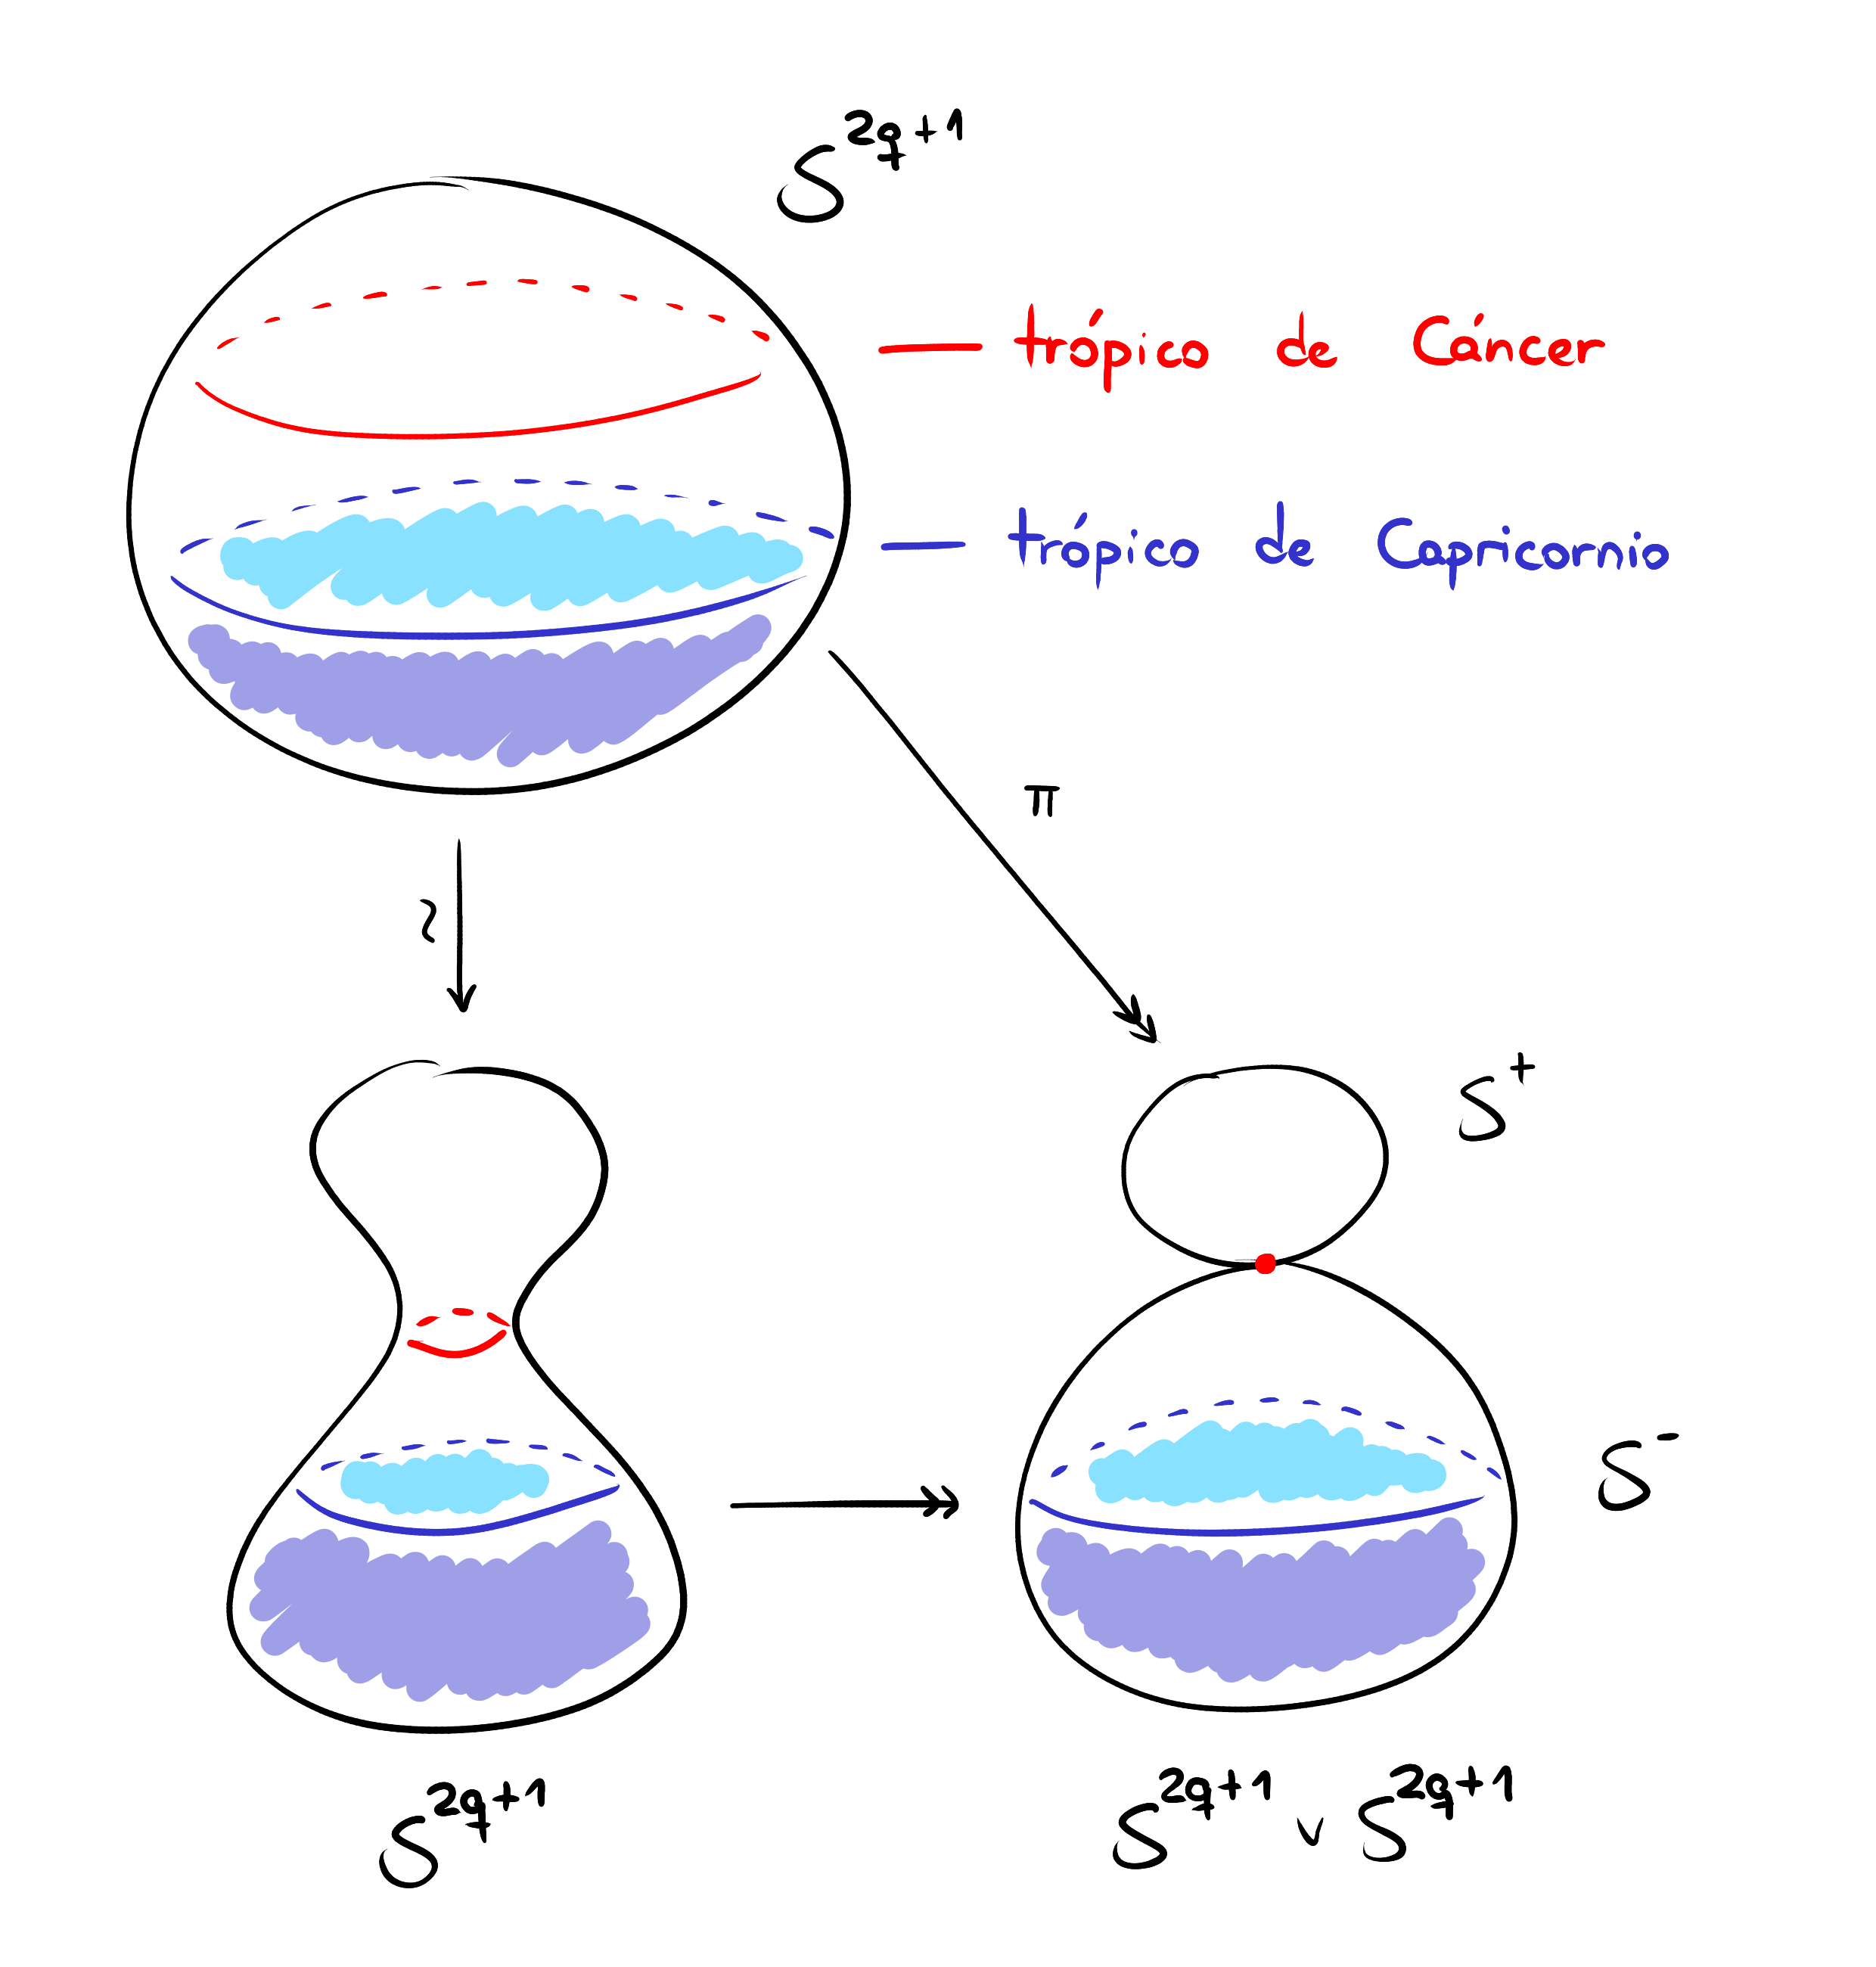
\includegraphics[scale=0.20]{spheres.png}
    \caption {La proyección $\pi : S^{2q+1} \to S^{2q+1} \vee S^{2q+1}$.}
\end{figure}

Por hipótesis, $\phi_-$ ya está definida sobre $D^- = \pi(D^\sqcup)$. Para cerrar el diagrama
$$
\begin{tikzcd}[row sep = huge, column sep = huge]
    D^- \arrow[d, hook] \arrow[rd, "\widetilde \phi_-"] \\
    S^- \arrow[r, dashed, "\phi_-"] & V_k(\C^n),
\end{tikzcd}
$$
identifiquemos $D^-$ con el hemisferio sur de $S^-$ y definamos $\phi_- = \widetilde \phi_- \circ \beta$, donde $\beta : S^- \to D^-$ es la función que refleja el hemisferio norte de $S^-$ a través del plano ecuatorial. Entonces,
$$[\phi_-] = [\widetilde \phi_-] \circ \cancelto 0 {[\beta]} \, \, \, = 0$$
es el elemento neutro de $\pi_{2q+1} \circ V_k(\C^n)$.

Tomemos ahora un representante arbitrario $\psi : S^+ \longrightarrow V_k(\C^n)$ de la clase $d(e_\alpha)$. Usando un cambio de base $g \in \GL_n(\C)$, identifiquemos $g \circ \psi(p_0) = \phi_-(p_0)$, de tal manera que $\phi_+ = g \circ \psi$ y $\phi_-$ se puedan pegar. Puesto que $\GL_n(\C)$ es conexo, tenemos
$$
[f_\alpha]
    = [\phi \circ \pi]
    = [\phi_+ \vee \phi_-]
    = [\phi_+] + \cancel {[\phi_-]}
    = [g \circ \psi]
    = \cancel {[g]} \cdot [\psi]
    = d(e_\alpha).
$$
Por lo tanto, $\rho$ es la homotopía hueca solicitada y la diferencia
$$c(\sigma) - \delta d(\rho) = c(\sigma) - \delta d$$
es el cociclo de obstrucción de la sección de $V^{2q+1}$ definida sobre $M^{2q+1} \times \{ 1 \}$.
\end{proof}
